 \section{Normalisation ODP}\begin{description}
\item [ALSO KNOWN AS:] Untangling.

\item [CLASSIFICATION:] Good Practice.

\item [MOTIVATION:] There are ontologies where a given class can have plenty of superclasses, building a polyhierarchy. If all those subsumption relationships are directly stated by the ontology maintainer, two main problems rise: (i) the ontology becomes very difficult to maintain: whenever a subsumption must be deleted (because a class has changed) or created (because a new class has been created) it has to be done by hand; in a polyhierarchy the process becomes very inefficient and error-prone. (ii) the semantics are implicitly stated, not explicitly: any other ontologist or reasoner only knows that a class is a subclass of its superclasses, without knowing why.

\item [AIM:] To untangle a polyhierarchy, coding the subsumption relationships using restrictions rather than class-subclass relationships. The application example for this ODP is adapted from the Cell Type Ontology. In the example, the subsumption relationships that already are in the Cell Type Ontology are inferred by the reasoner instead of hard-coded. The term Neutrophil is used as an example class to show how a class can relate to different modules.

\item [STRUCTURE:] See Figure \ref{odp:Normalisation_abstract}.
\begin{figure}[]\centering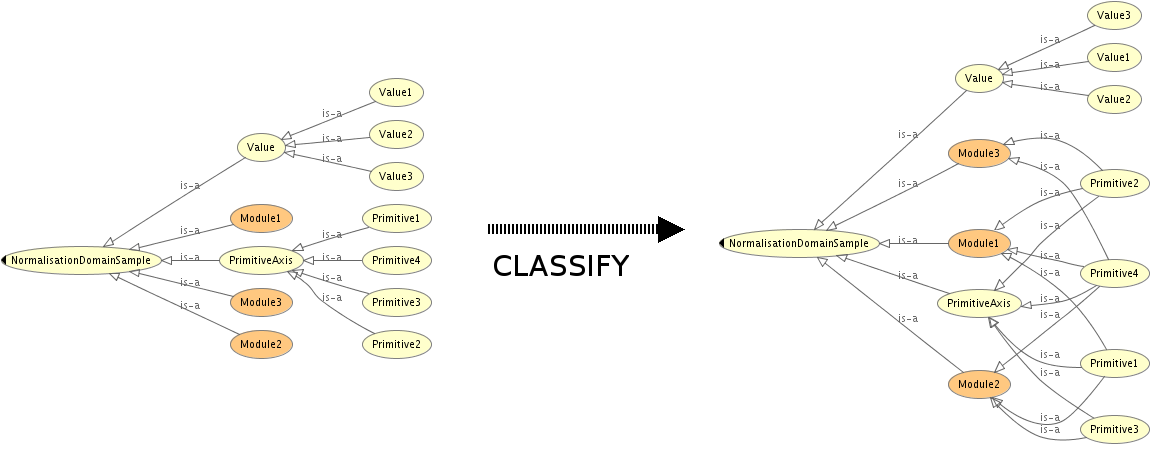
\includegraphics[width=\textwidth]{Catalogue/Normalisation_abstract}\caption{\label{odp:Normalisation_abstract} Abstract structure of the Normalisation ODP.}\end{figure}

\item [SAMPLE:] See Figure \ref{odp:Normalisation_instance}.
\begin{figure}[]\centering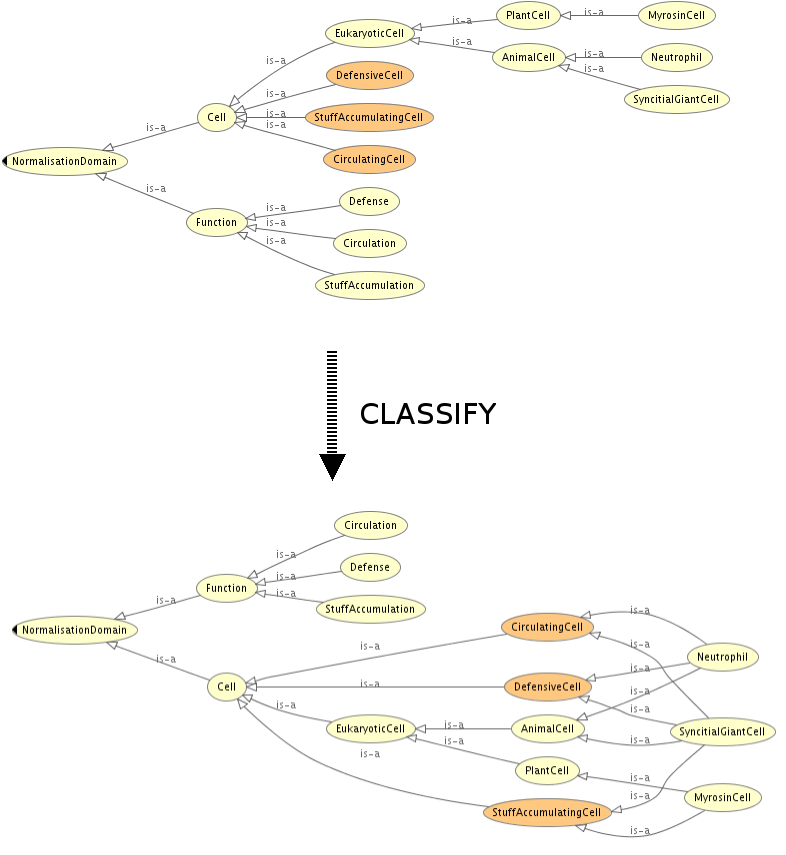
\includegraphics[width=\textwidth]{Catalogue/Normalisation_instance}\caption{\label{odp:Normalisation_instance} Sample structure of the Normalisation ODP.}\end{figure}

\item [ELEMENTS:] The original classes of the ontology are divided in different axes. The conditions for each subsumption relationship are encoded as restrictions (e.g. [PerformsFunction some Defense]) that will relate the different modules.

\item [IMPLEMENTATION:] Identify the modules: group the classes. Create the modules, maintaining only one parent for any given primitive class and making primitive siblings disjoint. Redefine the classes (or define the newly added classes) according to the conditions for belonging to each module. Protege includes a wizard, the restrictions matrix, that helps in the process.

\item [RESULT:] The ontology gets untangled and becomes a collection of neat modules. The rest of the semantics are given by restrictions pointing to the modules, and the reasoner maintains the structure, avoding error-prone human maintenance of the polyhierarchy.

\item [REFERENCES: ] ~\begin{itemize}
\item Alan L. Rector. Modularisation of Domain Ontologies Implemented in Description Logics and related formalisms including OWL. K-CAP 2003.
\item Alan L. Rector, Chris Wroe, Jeremy Rogers and Angus Roberts. Untangling Taxonomies and Relationships: personal and Practical Problems in Loosely Coupled Development of Large Ontologies. K-CAP 2001.
\item \url{http://www.co-ode.org/resources/tutorials/bio/}\end{itemize}
\item [URL: ] \url{http://www.gong.manchester.ac.uk/odp/owl/Good_Practice_ODP/Normalisation.owl} \end{description}